%------------------------------- JPADCAD module --------------------------------
\chapter{\texttt{JPADCAD} module}
\label{chap2}

%------------------------------- CAD: motivations and approaches --------------------------------
\section{CAD: motivations and approaches}
\label{sec2.1}

In paragraph \ref{sec1.2}, it was mentioned why the generation of a 3D \gls{CAD} model in a software such as \gls{JPAD} could prove particularly useful. In this section the attention will be focused even more on the motivations that may lead to the need to generate a complete 3D model of the aircraft even in the initial design stages. 

\bigskip
\noindent
\gls{CFD} has increasingly become, over the last three decades, an indispensable tool for aerodynamic studies in aircraft design. Nowadays, viscous \gls{CFD} simulations are carried out in ever increasing numbers and at all stages of the design. \gls{CFD} is particularly useful in terminal project stages, when simulations are required in the most disparate phases of flight (such as take-off or landing). With the possibility of producing unstructured mesh, the spectrum of \gls{CFD} applications has expanded further, and, at the moment, there seem to be no limits to the geometric complexity that can be fed to \gls{CFD} solvers. This also happens thanks to the continouos reduction of the time needed to create the mesh and perform the calculations. Engineers can now perform complex simulations using a simple desktop computer, when, on the other hand, the same simulations would have required a cluster for parallel computing only a few years ago. This growing computing power has given engineers the ability to carry out most of the design and analysis work of complex systems without the need to resort to physical models or prototypes.

\bigskip
\noindent
Nowadays there is an ever increasing demand in the aerospace industry to use \gls{CFD} analysis even in the preliminary and conceptual phases of aircraft design. This is due to the fact that \gls{CFD} simulations can predict the compressible and viscous flow fields around the aircraft taking into account all the important aerodynamic phenomena. The result is the achievement of forces on points on the surfaces or integral forces for each of the components of the aircraft. These forces will take into account viscous and transonic phenomena and interferences between components, with a reliable accuracy. Moreover, in the cases in which it is desired to analyze new and uncommon configurations, the estimation of certain aerodynamic characteristics through the traditional techniques of the preliminary design phase could be difficult or completely impossible. This is because many of these methods, of an empirical or semiempirical nature, have been conceived and calibrated for use in the case of classical or ordinary configurations. In this case, the \gls{CFD} analysis would come to the rescue, limiting the risks of making gross errors in the early design phases. \cite{paperCADinAero} 

\bigskip
\noindent
But aerodynamics is not the only domain that needs to be investigated. In a multi-disciplinary design context, such as that of aircraft design, engineers have to deal with different disciplines at the same time, and necessitate to make sure the solutions they come up to are the closest possible to the optimum ones. Traditionally, in the early stages of design, engineers are in possess of what is defined as the \gls{acr:OML} of the aircraft, and the details of other subsystems, such as structural layouts, are not examined until later design phases. But, in general, the configuration's \gls{acr:OML} geometry design is impacted by these subsystems, and it may be not discovered until high-fidelity analyses are performed in later development phases. Besides, further complications could arise whenever the geometry definition is scattered over many different analysis methods, which can span different disciplines as well as different fidelity levels within a discipline. What could happen is that geometry adjustments from redesign based on one method are likely to be inconsistent with the other geometry definitions. One solution to these difficulties and complications is, again, to generate a 3D model of the aircraft much earlier during the design study, as during the preliminary or even the conceptual phase, and to use this 3D model for all the possible analyses. Having a 3D model at disposal during conceptual design phase and performing on it higher fidelity analyses (alongside low-fidelity ones) would lead to a greater confidence in calculated data and for configuration down-select. Besides, there would be no need to generate new and more precise geometries as the design process progresses, because the 3D model of the aircraft would mature during the design process itself. \cite{AIAApaperHaimesDrela}

\bigskip
\noindent
What appears quite clear from the previous examination is that the performing of high-fidelity analyses is something really auspicable even during the first stages of the aircraft design process. But, in order to perform these analyses, an adequate geometry generator must be used. At this stage several approaches can be considered, especially when parametrization and \gls{MDO} need to be taken into account. 

\bigskip
\noindent
A \gls{acr:FFD} volume approach for \gls{CAD}-free geometry parametrization can be followed, as presented in \cite{AIAApaperKenwayKennedy}. The \gls{acr:FFD} approach is borrowed directly from soft object animation in the computer graphics field and allows to perform high level modifications to complex objects by simply embedding them in a rubber-like volume, which is stretched and twisted in order to obtain, indirectly, the desired final shape for the object (figure \ref{fig:FFD}). One key observation that needs to be made about \gls{acr:FFD} is that it parametrizes not the geometry itself, but the geometry change. This brings to an efficient computation of analytic derivatives for gradient-based optimization.
%
\begin{figure}[H]
\centering
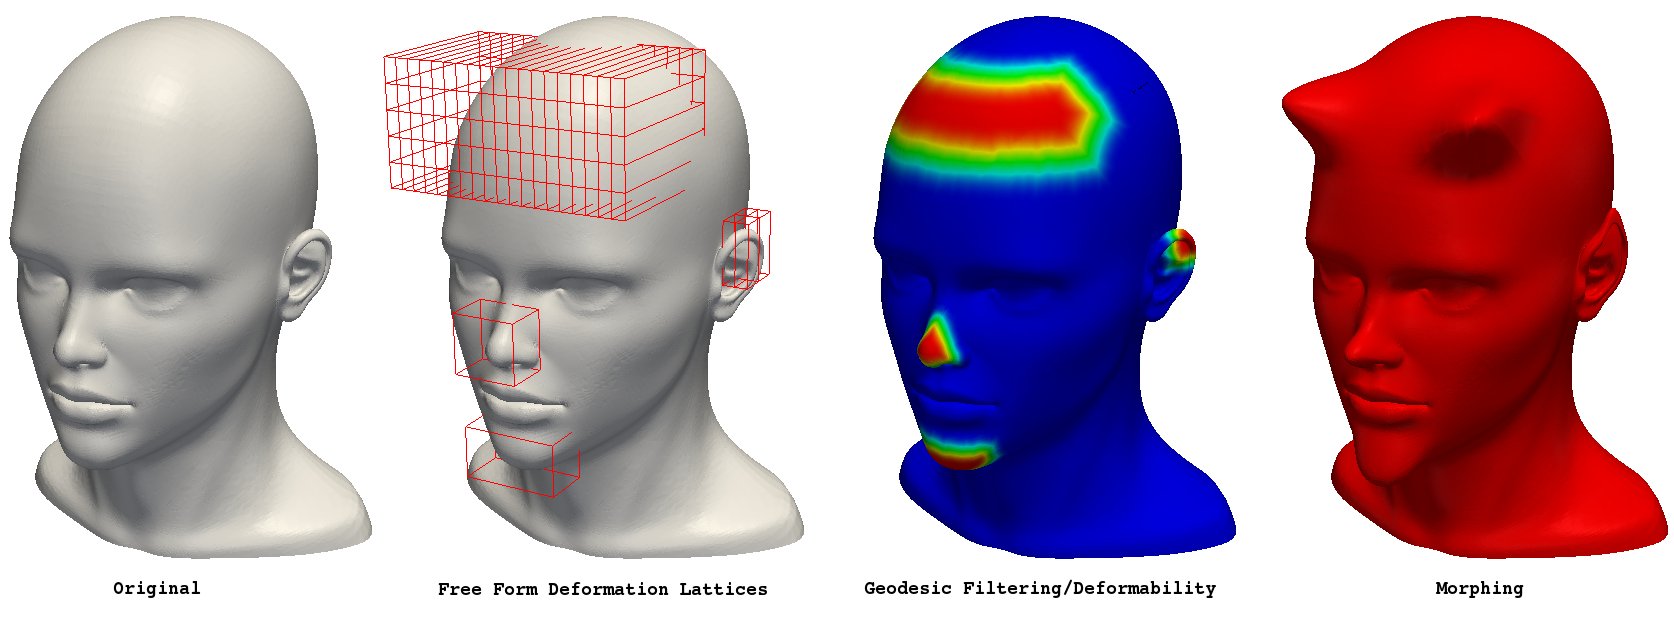
\includegraphics[scale=1.05]{Immagini/Capitolo2/ffdprocedure}
\caption{Free-form deformation example (\href{www.optimad.it/wp-content/uploads/ffdprocedure.png}{www.optimad.it/wp-content/uploads/ffdprocedure.png})}
\label{fig:FFD}
\end{figure}
%

\bigskip
\noindent
A further approach to the problem is described in \cite{paperCADinAero}, in which the author examines the potential of parametric \gls{CAD} systems and the help they can offer during the early stages of aircraft design. In a parametric CAD software, contrary to what happens in conventional \gls{CAD} systems, at each step the user has the possibility to name the entity that is being created and to make a parameter one or more values of the entity itself. In the event that one of the parameters is changed, all the child entities of the element to which the mutated parameter belongs are updated.

\bigskip
\noindent
One last possible approach is the one used in \cite{AIAApaperHaimesDrela}, which involves the generation of a general geometry \gls{acr:API} in order to create solids-based geometries. In particular, the \gls{acr:API} created by the authors (named EGADS) provides a solid modeling geometry kernel that supports both \emph{Bottom-Up} construction (i.e., the process of producing a solid model from its constituent geometric entities) as well as the ability to perform \gls{CSG} operations. Both capabilities are necessary in order to build closed 3D models, which are essentials for high-fidelity analyses. The core of EGADS is Open CASCADE, a fully functional open-source solid modeling geometry kernel, which incorporates all the methods and operations necessary to perform shape manipulation. Since the approach is \emph{Bottom-Up} and programmatic (each of the geometric and topological entities is assigned one or more manageable variables) the 3D \gls{CAD} models produced will be, to a certain extent, parametrized \emph{a priori}. As it will be more clear from the following paragraphs, the approach used for \gls{JPAD} is pretty similar to the latter.

%------------------------------- Open CASCADE Technology --------------------------------
\section{Open CASCADE Technology}
\label{sec2.2}

As anticipated in section \ref{sec2.1}, the \lstinline[language=Java]!JPADCAD! module helps the user to build from scratch, in a \emph{Bottom-Up} approach, aircraft solid components ready to be passed to a \gls{CFD} solver, in order to perform high-fidelity analysis. This would have not been possible without the adoption of an external library such as \gls{OCCT}.

\bigskip
\noindent
Open CASCADE Technology (\gls{OCCT}) is an object-oriented C++ class library designed for rapid production of sophisticated domain-specific \gls{CAD} applications. A typical application developed using \gls{OCCT} deals with 2/3D geometric modeling in general-purpose or specialized \gls{CAD} systems, manifacturing or analysis applications, simulations applications, or even illustration tools. \gls{OCCT} provides classes for several purposes, such as:
%
\begin{itemize}
\item basic data structures (e.g., geometric modeling, visualization, interactive selection);
\item modeling algorithms;
\item working with mesh;
\item data interoperability with neutral formats, such as IGES and STEP.
\end{itemize}
%
The C++ classes are located into packages, which are organized into toolkits, which are finally grouped into seven modules \cite{webOpenCASCADE} (figure \ref{fig:OCCTStructure}):
%
\begin{itemize}
\renewcommand\labelitemi{\tiny$\blacksquare$}
\item \textbf{Foundation Classes} module underlies all other \gls{OCCT} classes;
\item \textbf{Modeling Data} module supplies data structures to represent 2D and 3D geometric primitives and their compositions into \gls{CAD} models;
\item \textbf{Modeling Algorithms} module contains a wide range of geometrical and topological algorithms;
\item \textbf{Mesh} module implements tessellated representation of objects;
\item \textbf{Visualization} module provides mechanisms for graphical data representation;
\item \textbf{Data Exchange} module interacts with popular data formats and relies on \textbf{Shape Healing} module to improve compatibility between different \gls{CAD} software;
\item \textbf{Application Framework} module offers solutions for handling application-specific data and commonly used functionality (e.g., save/restore, undo/redo, copy/paste).
\end{itemize}
%
In addition, Open CASCADE comes equipped with a convenient testing tool, called \textbf{Test Harness} or \textbf{Draw}, that can be used to test and prototype various algorithms before building an entire application.
%
\begin{figure}[H]
\centering
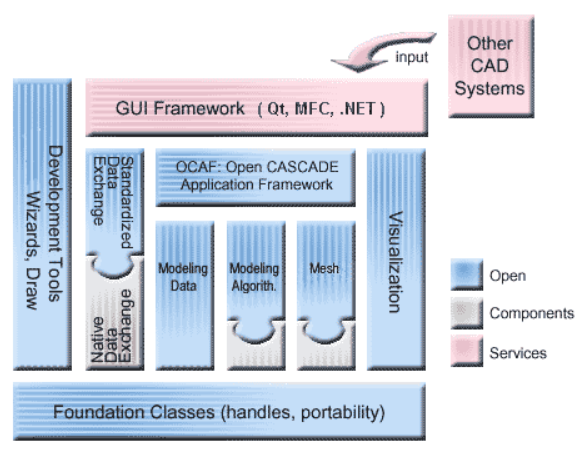
\includegraphics[scale=2.0]{Immagini/Capitolo2/OCCTStructure}
\caption{OCCT module structure}
\label{fig:OCCTStructure}
\end{figure}
%
\noindent
In the following subsections more will be said about the Modeling Data module, the Modeling Algorithms module, and the Data Exchange module, because these are the packages which group the majority of the classes used within \lstinline[language=Java]!JPADCAD!.

\subsection{Modeling Data and Algorithms}
\label{sec2.2.1}

Modeling Data module supplies data structures to implement \gls{BRep} of objects in three dimensions. In \gls{BRep} each shape is an aggregation of geometry within topology. The geometry is the mathematical description of a shape, and it is given by curves and surfaces, which can be of different types (e.g., Bezier, B-Spline, \gls{acr:NURBS}). The topology is a data structure binding geometrical objects together. 

\bigskip
\noindent
On the other hand, Modeling Algorithms module groups a wide range of topological and geometric algorithms used in modeling. These algorithms can be divided in two major groups. The first one comprehends high-level routines used in the real design, such as primitives construction (e.g., boxes, prisms, cylinders), kinematic modeling (e.g., prisms, pipes,), Boolean operations, and algorithms for local modifications (such as hollowing and shelling). The second one groups low-level mathematical support functions, low-level geometric tools, and topological tools providing algorithms to tesselate shapes, convert shapes to \gls{acr:NURBS} geometry, sew connected topologies, etc.

\subsubsection{Geometry}

Geometric entities are grouped in two packages: \lstinline[language=Java]!Geom2d! and \lstinline[language=Java]!Geom!. As the names suggest, \lstinline[language=Java]!Geom2d! package defines geometric objects in 2D space, while \lstinline[language=Java]!Geom! package deals with geometric entities in three dimensions. These packages provide classes for:
%
\begin{itemize}
\renewcommand\labelitemi{$\bullet$}
\item description of points, vectors, curves and surfaces (just \lstinline[language=Java]!Geom!, for obvious reasons);
\item their positioning in the plane/space using coordinates systems;
\item their geometric transformation, by applying translations, rotations, symmetries, scaling transformations and combinations thereof.
\end{itemize}
%
The following geometric objects are available in \gls{OCCT}, with the last four entities pertaining to the \lstinline[language=Java]!Geom! package:
%
\begin{itemize}
\renewcommand\labelitemi{$\bullet$}
\item point,
\item vector,
\item direction,
\item axis,
\item line,
\item conic (circle, ellipse, hyperbola, parabola),
\item bounded curve (trimmed curve, Bezier curve, \gls{acr:NURBS} curve),
\item offset curve,
\item elementary surface (plane, cylinder, cone, sphere, torus),
\item bounded surface (rectangular trimmed surface, Bezier surface, \gls{acr:NURBS} surface),
\item swept surface (surface of linear extrusion, surface of revolution),
\item offset surface.
\end{itemize}
%
One peculiar characteristic of \lstinline[language=Java]!Geom! curves and surfaces is that they are parametrized. For this reason each class comes equipped with functions that allow the user to work with the parametric equation of the curve or surface and to compute the point of a certain parameter u on a curve or the points of parameter $(\text{u}, \text{v})$ on a surface, together with the derivatives (in form of vectors) of every order at this point.

\subsubsection{Topology}

\gls{OCCT} topology allows accessing and manipulating data of objects without dealing with their 2D or 3D representation. Whereas \gls{OCCT} geometry provides a description of objects in terms of coordinates or parametric values, topology describes data structures of objects in parametric space. These description use location in and restriction of parts of this space. Abstract topological data structure describes a basic entity (i.e., a shape), which can be divided into the following component topologies.
%
\begin{itemize}
\renewcommand\labelitemi{\tiny$\blacksquare$}
\item \textbf{Vertex}: a zero-dimensional shape which correspond to a point in geometry.
\item \textbf{Edge}: a shape corresponding to a curve, and bound by a vertex at each extremity.
\item \textbf{Wire}: a sequence of edges connected by their vertices.
\item \textbf{Face}: part of a surface bounded by a closed wire.
\item \textbf{Shell}: a collection of faces connected by some edges of their wire boundaries.
\item \textbf{Solid}: a part of 3D space bound by a shell.
\item \textbf{Solids Compound}: a collection of solids.
\end{itemize}
%
\gls{OCCT} topology is provided by six packages. In the following list, the first three packages describe the topological data structure used in Open CASCADE Technology, while the remaining three provide tools to access and manipulate this topology.
%
\begin{itemize}
\renewcommand\labelitemi{\tiny$\blacksquare$}
\item \textbf{\lstinline[language=Java]!TopAbs!} package groups all the necessary resources for topology-driven applications. It contains enumerations that are used to describe basic topological notions, like topological shape, orientation and state. It also provides methods to manage these enumerations.
\item \textbf{\lstinline[language=Java]!TopLoc!} package provides resources useful to handle 3D local coordinates systems.
\item \textbf{\lstinline[language=Java]!TopoDS!} package contains classes to model and build data structures that are purely topological.
\item \textbf{\lstinline[language=Java]!TopTools!} package provides basic tools to use on topological data structures.
\item \textbf{\lstinline[language=Java]!TopExp!} package provides classes to explore and manipulate the topological data structures contained in the \lstinline[language=Java]!TopoDS! package.
\item \textbf{\lstinline[language=Java]!BRepTools!} package provides classes to explore, manipulate, read and write \gls{BRep} data structures. These more complex data structures combine topological descriptions with additional geometric information, and include rules for evaluating equivalence of different possible representation of the same object.
\end{itemize}
%

\subsubsection{Geometry Utilities}

In order to manage geometry, there are several utilities which provide the following services. Just a few of these tools is contained in the Modeling Data package, while the majority is located in the Modeling Algorithms one.
%
\begin{itemize}
\renewcommand\labelitemi{\tiny$\blacksquare$}
\renewcommand\labelitemii{\tiny$\bullet$}
\item \textbf{Creation of shapes by interpolation and approximation}. In modeling, it is often required to approximate or interpolate points into curves and surfaces. In interpolation, the process is complete when the curve or surface passes through all the points; in approximation, when it is as close to these points as possible. In Open CASCADE, these processes can be performed both in 2D and in 3D, providing the interpolator/approximator method a set of 2D or 3D points. In particular, packages \lstinline[language=Java]!Geom2dAPI! and \lstinline[language=Java]!GeomAPI! provide simple methods for approximation and interpolation with minimal programming. Different types of approximator/interpolator curves can be obtained, such as B-Spline, Bezier and \gls{acr:NURBS}, by simply selecting the right options.
\item \textbf{Direct construction of shapes}. Direct construction methods from \lstinline[language=Java]!gce!, \lstinline[language=Java]!GC! and \lstinline[language=Java]!GCE2d! packages provide algorithms to build elementary geometric entities, such as lines, circles and curves. They complement the reference definitions provided by the \lstinline[language=Java]!gp!, \lstinline[language=Java]!Geom! and \lstinline[language=Java]!Geom2d! packages. The algorithms implemented by \lstinline[language=Java]!gce!, \lstinline[language=Java]!GC! and \lstinline[language=Java]!GCE2d! are simple: there is no creation of objects defined by advanced positional constraints. For example, to construct a circle one could simply provide a point and a radius. The above mentioned simple entities that can be created comprehend:
	%
	\begin{itemize}
	\item 2/3D lines,
	\item 2/3D conics (circles, ellipses, hyperbolae, parabolae),
	\item arcs (of circle, ellipse, parabola, hyperbola),
	\item planes,
	\item cylinders,
	\item cones,
	\item transformations.
	\end{itemize}
	%
\item \textbf{Conversion of curves and surfaces to B-Spline curves and surfaces}. The conversion to and from B-Spline has two distinct purposes. The first one is to provide a homogeneous formulation which can be used to describe any curve or surface. The second one is that it can be used to divide a B-Spline curve or surface into a series of curves or surfaces, thereby providing a higher degree of continuity. All these utilities are grouped in two packages: \lstinline[language=Java]!Geom2dConvert! and \lstinline[language=Java]!GeomConvert!.
\item \textbf{Computation of the coordinates of points on 2D and 3D curves}. \gls{OCCT} gives the user the possibility to use complex algorithms that compute points on a 2D or 3D curve. For example, the following characteristic points exist on parametrized curves in 3D space:
	%
	\begin{itemize}
	\item points equally spaced on a curve,
	\item points distributed along a curve with equal chords,
	\item a point at a given distance from another point on a curve.
	\end{itemize}
	%
Even more options become available by the use of dedicated packages, such as \lstinline[language=Java]!GCPnts!.
\item \textbf{Calculation of extrema between shapes}. The classes to calculate the minimum distance between points, curves, and surfaces, both in 2D and 3D, are provided by \lstinline[language=Java]!Geom2dAPI! and \lstinline[language=Java]!GeomAPI! packages. These packages give the user the capability to calculate the extrema of distance between:
	%
	\begin{itemize}
	\item a point and a curve,
	\item a point and a surface,
	\item two curves,
	\item a curve and a surface,
	\item two surfaces.
	\end{itemize}
	%
\item \textbf{Calculation of intersections between shapes}. Four different types of intersection can be calculated in \gls{OCCT}:
	%
	\begin{itemize}
	\item the intersections between two 2D curves;
	\item the self-intersections of a 2D curve;
	\item the intersection between a 3D curve and a surface;
	\item the intersection between two surfaces.
	\end{itemize}
	%
Intesection between curves in 2D space is managed by the \lstinline[language=Java]!Geom2dAPI_InterCurveCurve! class, while, in 3D space, the intersection between a curve and a surface and two different surfaces is managed, respectively, by the \lstinline[language=Java]!GeomAPI_InterCS! class and the \lstinline[language=Java]!GeomAPI_InterSS! classes.
\item \textbf{Construction of 2D lines and circles from constraints}. \gls{OCCT} provides methods to build, in 2D space, circles and lines using numeric or geometric constraints in relation to other curves. These constraints can impose the following:
	%
	\begin{itemize}
	\item the radius of a circle,
	\item the angle that a straight line makes with another straight line,
	\item the tangency of a straight line or circle in relation to a curve,
	\item the passage of a straight line or circle through a point,
	\item the circle with center in a point or curve.
	\end{itemize}
	%
These algorithms are much more complex than the ones described in the Direct Construction section.
\item \textbf{Construction of curves and surfaces from constraints}. High level functions can be used in \gls{OCCT} in order to create faired and minimal variation 2D curves (\lstinline[language=Java]!FairCurve! package), ruled, pipe and filling of surfaces (\lstinline[language=Java]!GeomFill! package), and plate surfaces (\lstinline[language=Java]!GeomPlate! package).
\item \textbf{Computation of projections}. \gls{OCCT} provides algorithms in order to compute:
	%
	\begin{itemize}
	\item the projections of a 2D point onto a 2D curve;
	\item the projections of a 3D point onto a 3D curve or surface;
	\item the projection of a 3D curve onto a surface.
	\end{itemize}
The classes providing these services are grouped in the \lstinline[language=Java]!Geom2dAPI! and \lstinline[language=Java]!GeomAPI! packages.
\end{itemize}
%

\subsubsection{Topology Tools and Algorithms}

In order to generate topological entities starting from geometric objects or other entities of topological type, the Modeling Algorithms package is provided with different sub-packages, each one specialized in a specific domain. These packages are as follows.
%
\begin{itemize}
\renewcommand\labelitemi{\tiny$\blacksquare$}
\renewcommand\labelitemii{\tiny$\bullet$}
\item \textbf{\lstinline[language=Java]!BRepBuilderAPI!} - Provides classes in order to create \gls{BRep} topology data structure. The \lstinline[language=Java]!BRepBuilderAPI_MakeShape! class is the root of all \lstinline[language=Java]!BRepBuilderAPI! classes, which build shapes. In order to generate an edge element, for example, a \lstinline[language=Java]!BRepBuilderAPI_MakeEdge! object will be created, providing several methods to build an edge from a curve. The \lstinline[language=Java]!BRepBuilderAPI! package also provides classes which allow the creation of connected topology (shells and wires) from a set of separate topological elements (faces and edges). The sewing algorithm is implemented in the class \lstinline[language=Java]!BRepBuilderAPI_Sewing!, which provides methods to load initial data, set customization parameters (such as tolerances), apply analisys methods, and sew the loades shapes.
\item \textbf{\lstinline[language=Java]!BRepFilletAPI!} - Provides classes in order to create fillets and chamfers. A fillet is a smooth face replacing a sharp edge and the class which allows filleting a shape is \lstinline[language=Java]!BRepFilletAPI_MakeFillet!. To produce a fillet it is necessary to define the filleted shape at the construction of the class and add fillet descriptions (such as the radius) using the \lstinline[language=Java]!Add! method. Fillet with changing radius can be also created. On the other hand, a chamfer is a rectilinear edge replacing a sharp vertex of the face and can be performed by using the \lstinline[language=Java]!BRepFilletAPI_MakeChamfer! class. The procedure to produce a chamfer is almost equal to the one for the fillet construction.
\item \textbf{\lstinline[language=Java]!BRepOffsetAPI!} - It groups classes providing the following services:
	%
	\begin{itemize}
	\item creation of offset shapes and their variants, such as hollowing, shelling and lofting;
	\item creation of tapered shapes using draft angles;
	\item creation of sweeps (i.e., objects obtained by sweeping a profile along a path).
	\end{itemize}
	%
\item \textbf{\lstinline[language=Java]!BRepPrimAPI!} - Provides classes for primitives construction, such as boxes, cones, cylinders and prisms. These classes also allow to create partial solids, such as a sphere limited by longitude, and build specific sub-parts by sweeping along a profile (altough for swept constructions along complex profiles such as B-Spline curves the \lstinline[language=Java]!BRepOffsetAPI! package shoul be preferred).
\item \textbf{\lstinline[language=Java]!BRepAlgoAPI!} - This package mainly deals with Boolean operations. Boolean operations are used to create new shapes from the combinations of two shapes. These operations are the most convenient way to create real industrial parts. As most industrial parts consist of several simple elements such as gear wheels, arms, holes, ribs, tubes and pipes, it is usually easy to create those elements separately and then to combine them by Boolean operations in the whole final part. Four operations can be performed, provided by five main classes, of which one (\lstinline[language=Java]!BRepAlgoAPI_BooleanOperation!) is the root:
	%
	\begin{itemize}
	\item \lstinline[language=Java]!BRepPrimAPI_Fuse! performs the fuse operation;
	\item \lstinline[language=Java]!BRepPrimAPI_Common! performs the common operation;
	\item \lstinline[language=Java]!BRepPrimAPI_Cut! performs the cut operation;
	\item \lstinline[language=Java]!BRepPrimAPI_Section! performs the section operation, whose result is a compound made of edges.
	\end{itemize}
	%
In general, Boolean operations can be performed in \gls{OCCT} for various types of arguments. For arguments having the same shape type, for example, the result is a compound, containing shapes of this type. In case of different shape type arguments, some boolean operations can not be performed. For example, the fuse operation between a shell and a solid can not be done, while the cut operation can be performed, provided that the shell is the argument (i.e., the object of the operation) and the solid is the tool.
\item \textbf{\lstinline[language=Java]!BRepFeat!} - This package helps the user for creation and manipulation of form and mechanical features that go beyond the classical boundary representation of shapes. The form features are depressions or protrusions including types such as cylinders, prisms and pipes.
\end{itemize}

\subsection{Data Exchange}
\label{sec2.2.2}

Data Exchange module allows developing \gls{OCCT}-based applications that can interact with other \gls{CAD} systems by writing and reading \gls{CAD} models to and from external data. The exchanges run smoothly regardless of the quality of external data or requirements to its internal representation, for example, to the data types, accepted geometric inaccuracies, etc. Data Exchange module is organized as a set of interfaces that comply with various \gls{CAD} formats: IGES, STEP, STL, VRML, etc. These interfaces allow software based on \gls{OCCT} to exchange data with various \gls{CAD} software packages, mantaining a good level of interoperability.
%
\begin{itemize}
\renewcommand\labelitemi{\tiny$\blacksquare$}
\renewcommand\labelitemii{\tiny$\bullet$}
\item \textbf{Standardized Data Exchange} interfaces allow querying and examining the input file, converting its contents to a \gls{CAD} model and running validity checks on a fully translated shape. The following formats are currently supported:
	\begin{itemize}
	\item STEP (AP203: Mechanical Design; AP214: Automotive Design),
	\item IGES (up to 5.3),
	\item VRML and STL meshes.
	\end{itemize}
\item \textbf{Extended Data Exchange} (XDE) allows translating additional attributes attached to geometric data (colors, layers, names, materials, etc.).
\item \textbf{Advanced Data Exchange Components} are available in addition to Standard Data Exchange interfaces to support interoperability and data adaptation with \gls{CAD} software using the following proprietary formats:
	\begin{itemize}
	\item ACIS SAT,
	\item Parasolid,
	\item DXF.
	\end{itemize}
\end{itemize}
%

\subsection{Open CASCADE Technology Java Wrapper}
\label{sec2.2.3}

The \gls{OCCT} classes are natively written in C++, while \gls{JPAD} is a program written in Java. In order to be able to use the \gls{OCCT} classes in \gls{JPAD}, it is necessary to use a tool that links the two languages. For this purpose, Open CASCADE offers its own Java Wrapper, a tool for wrapping Open CASCADE Technology C++ classes to Java language, to allow their use within Java applications. In particular, the wrapping is made using the \gls{SWIG} tool \cite{webSWIG}. \gls{SWIG} is an interface compiler that connects programs written in C and C++ with languages such as Perl, Python, Java, etc. It works by taking the declarations found in C/C++ header files and using them to generate the wrapper code that other languages need to access the undelying C/C++ code. The Open CASCADE Java Wrapper comes equipped with the \gls{SWIG} interface file (occtypes.i), which contains definitions of basic \gls{OCCT} types for \gls{SWIG} and defines several \gls{SWIG} macros facilitating wrapping of other \gls{OCCT} types. For example, the \texttt{WRAP_AS_ENUM_INCLUDE(name)} macro is uded to wrap enumerations, while \texttt{WRAP_AS_PACKAGE(name)} is used to wrap package methods. The use of these macros allows blind yet customizable approach to wrapping, facilitating controllable but easy wrapping of everything what is needed. The \gls{OCCT} \gls{acr:SDK} currently in use along with the Java wrapper is the 7.0.0 version, altough, at the moment this document is being written, the most recent version is the 7.3.0.

%------------------------------- JPADCAD structure --------------------------------
\section{\texttt{JPADCAD} structure}
\label{sec2.3}

The Open CASCADE Technology library is extremely useful for various reasons, which can be listed as follows:
%
\begin{itemize}
\item supports Manifold and Non-\gls{manifold:geometry};
\item gives the user the possibility to perform \emph{Bottom-Up} construction;
\item has both \gls{CSG} operations and other abstract \emph{feature-like} construction methods;
\item can read and write IGES, STEP and native file formats;
\item is a fully object-oriented \gls{acr:API} with thousands of methods and millions of lines of code.
\end{itemize}
%
The last point is both an advantage and a disadvantage. Having a plethora of methods to chose from surely gives the users all they necessitate to realize the most various applications. On the other hand, the level of programming complexity with the huge suite of methods makes the use of Open CASCADE rather a difficult undertaking. Moreover, its lack of a complete documentation adds to the enormous task of understanding this large but capable software suite. 

\bigskip
\noindent
All of these issues provide the motivation for the design and the development of a system of classes, interfaces and utilities which wrap the original \gls{OCCT} classes, allowing the current and future \gls{JPAD} developers to deal with a lowest number of well documented methods and functions, ready to be used in aerospace \gls{CAD} modeling. The following paragraphs deal with the structure of this system, which, it is good to clarify, is still under costant development. For this reason, some of the most advanced features (for example, those concerning Boolean operations) still need to be adequately wrapped and integrated into the \lstinline[language=Java]!JPADCAD! utilities superstructure.

\subsection{Abstract Factory pattern}
\label{sec2.3.1}

Most of the classes involved in the \gls{OCCT} library wrapping are in the shape domain. As for the \gls{OCCT} library, many topological entities must be managed at the same time in order to build solid models ready to be imported into external tools. The necessity to deal with many different entities all pertinent to the same domain as the possibility to employ, in the next future, geometric modeling kernels other than \gls{OCCT}, has led to the adoption, for the development of the \lstinline[language=Java]!JPADCAD! superstructure, of a particular \gls{design:pattern}. 

\bigskip
\noindent
By definition, \gls{design:pattern}s are reusable solutions to commonly occurring problems in the context of software design \cite{wikiDesignPatterns}. \gls{design:pattern}s were started as best practices that were applied again and again to similar problems encountered in different contexts. They became popular after they were collected, in a formalized form, in the Gang of Four book in 1994. The pattern adopted for \lstinline[language=Java]!JPADCAD! is the one that goes under the name of Abstract Factory pattern. The Abstract Factory pattern offers the interface for creating a family of related objects, without explicitly specifying their classes \cite{wikiAbstractFactoryPattern}. The classes that participate to the Abstract Factory pattern are the followings.
%
\begin{itemize}
\renewcommand\labelitemi{\tiny$\blacksquare$}
\item \textbf{\texttt{AbstractFactory}} - declares an interface for operations that create abstract products.
\item \textbf{\texttt{ConcreteFactory}} - implements operations to create concrete products.
\item \textbf{\texttt{AbstractProduct}} - declares an interface for a type of product object.
\item \textbf{\texttt{Product}} - defines a product to be created by the corresponding \texttt{ConcreteFactory}; it implements the \texttt{AbstractProduct} interface.
\item \textbf{\texttt{Client}} - uses the interfaces declared by \texttt{AbstractFactory} and \texttt{AbstractProduct} classes.
\end{itemize}
%
The \texttt{AbstractFactory} class is the one that determines the actual type of the concrete object and creates it, but it returns an abstract pointer to the concrete object just created. This determines the behavior of the \texttt{Client} that asks the factory to create an object of a certain abstract type and to return the abstract pointer to it, keeping the \texttt{Client} from knowing anything about the actual creation of the object. The fact that the factory returns an abstract pointer to the created object means that the client doesn't have knowledge of the object's type. This implies that there is no need for including any class declarations relating to the concrete type, the client dealing at all times with the abstract type. The objects of the concrete type, created by the factory, are accessed by the \texttt{Client} only through the abstract interface. Figure \ref{fig:AbstractFactoryUML} contains an \gls{acr:UML} diagram which shows how the pattern works. 
%
\begin{figure}[H]
\centering
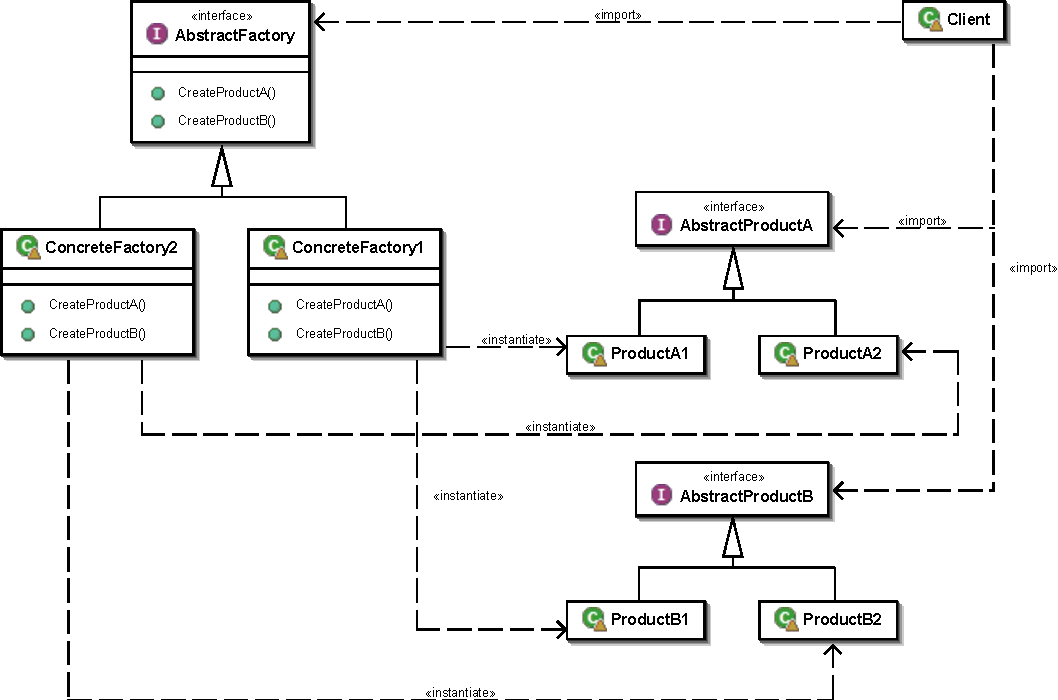
\includegraphics[scale=0.8]{Immagini/Capitolo2/Abstract_factory_UML}
\caption{Abstract Factory pattern \gls{acr:UML}}
\label{fig:AbstractFactoryUML}
\end{figure}
%
\noindent
As figure \ref{fig:AbstractFactoryUML} shows, the \texttt{Client} class that requires the \texttt{ProductA} and \texttt{ProductB} objects doesn't instantiate the \texttt{ProductA1} and \texttt{ProductB1} classes directly. Instead, the \texttt{Client} refers to the \texttt{AbstractFactory} interface for creating objects, which makes the \texttt{Client} independent of how the objects are created (i.e., which concrete classes are instantiated). The \texttt{ConcreteFactory1} class implements the \texttt{AbstractFactory} interface by instantiating the \texttt{ProductA1} and \texttt{ProductB1} classes. Obviously the same can be said for \texttt{ConcreteFactory2}, and \texttt{ProductA2} and \texttt{ProductB2} classes.

\subsection{\texttt{JPADCAD} classes and utilities}
\label{sec2.3.2}

The organizational structure of the \lstinline[language=Java]!JPADCAD! package follows the Abstract Factory pattern paradigm. In the specific case under examination, the abstraction from which all the classes of the package derive consists in considering the package itself as the superstructure of a generic (not better specified) kernel for \gls{CAD} modeling. Therefore, all the classes of the package that have the \lstinline[language=Java]!CAD! prefix are abstract classes (\lstinline[language=Java]!interface! or \lstinline[language=Java]!abstract class! reference types in Java) which therefore need to be implemented. Back to the Abstract Factory pattern, in the case of \lstinline[language=Java]!JPADCAD! the abstract factory is the abstract class \lstinline[language=Java]!CADShapeFactory!. As specified in the previous paragraph, the motivation that led to the use of the Abstract Factory pattern is the possibility that, in the future, more than just one kernel for geometric modeling could be used. Therefore, at present, being \gls{OCCT} the only \gls{CAD} library underlying \gls{JPAD}, the abstract factory \lstinline[language=Java]!CADShapeFactory! has a single implementation, consisting of the \lstinline[language=Java]!OCCShapeFactory! class. In general, all the \lstinline[language=Java]!JPADCAD! classes having the \lstinline[language=Java]!OCC! prefix are concrete classes related to the implementation of the \gls{OCCT} geometric modeling library.

\bigskip
\noindent
\lstinline[language=Java]!JPADCAD! currently comprises almost fourty classes, most of which are related to topological entities. More specifically, these classes can be distinguished as in table \ref{tab:JPADCADclasses}. 
%
\bigskip
\begin{table}[H]
\centering
\begin{tabular}{p{4.0cm}p{10.5cm}}
\toprule
\textbf{Class Type} & \textbf{Characteristics} \\
\midrule
Geometry classes & Define geometric entities (curve, surface) \\[0.5cm]
Shape classes & Define topological entities (vertex, edge, etc.) \\[0.5cm]
Factory classes & Provide factory methods \\[0.5cm]
Explorer classes & Define topological data structure explorers \\[0.5cm]
Iterator classes & Define iterators on sub-shapes \\[0.5cm]
Shape type classes & Provide type-safe enumeration of CAD types \\[0.5cm]
Utility classes & Provide methods to build/manipulate CAD entities \\[0.5cm]
JavaFX export classes & Provide data structure to import shapes into a JavaFX window \\
\bottomrule
\end{tabular}
\caption{\lstinline[language=Java]!JPADCAD! classes and characteristics}
\label{tab:JPADCADclasses}
\end{table}
%

\subsubsection{Shape classes}

Shape classes featured in \lstinline[language=Java]!JPADCAD! follow those offered by \gls{OCCT}, with table \ref{tab:JPADCADTopEnt} showing a comparison between the topology classes of Open CASCADE and the \gls{JPAD} ones. As the table reports, each topological entity has both an interface and its implementation. Moreover, each class specific to a particular topological entity (both interface and concrete class) extends a generic shape class, which is \lstinline[language=Java]!CADShape! for interface classes and \lstinline[language=Java]!OCCShape! for concrete classes. 
%
\bigskip
\begin{table}[H]
\centering
\begin{tabular}{ccc}
\toprule
\textbf{Open CASCADE} & \multicolumn{2}{c}{\textbf{JPAD}} \\
& \textbf{Abstract Topology} & \textbf{Concrete Topology} \\
\midrule
\lstinline[language=Java]!TopoDS_Shape! & \lstinline[language=Java]!CADShape! & \lstinline[language=Java]!OCCShape! \\
\lstinline[language=Java]!TopoDS_Vertex! & \lstinline[language=Java]!CADVertex! & \lstinline[language=Java]!OCCVertex! \\
\lstinline[language=Java]!TopoDS_Edge! & \lstinline[language=Java]!CADEdge! & \lstinline[language=Java]!OCCEdge! \\
\lstinline[language=Java]!TopoDS_Wire! & \lstinline[language=Java]!CADWire! & \lstinline[language=Java]!OCCWire! \\
\lstinline[language=Java]!TopoDS_Face! & \lstinline[language=Java]!CADFace! & \lstinline[language=Java]!OCCFace! \\
\lstinline[language=Java]!TopoDS_Shell! & \lstinline[language=Java]!CADShell! & \lstinline[language=Java]!OCCShell! \\
\lstinline[language=Java]!TopoDS_Solid! & \lstinline[language=Java]!CADSolid! & \lstinline[language=Java]!OCCSolid! \\
\lstinline[language=Java]!TopoDS_CompSolid! & \lstinline[language=Java]!CADCompSolid! & \lstinline[language=Java]!OCCCompSolid! \\
\lstinline[language=Java]!TopoDS_Compound! & \lstinline[language=Java]!CADCompound! & \lstinline[language=Java]!OCCCompound! \\
\bottomrule
\end{tabular}
\caption{\lstinline[language=Java]!JPADCAD! topology classes overview}
\label{tab:JPADCADTopEnt}
\end{table}
%
\noindent
Figure \ref{fig:OCCMap} gives a complete overview on how topology classes are related to each other. Being \lstinline[language=Java]!CADShape! a generic shape interface, it features basic methods common to all type of shapes. These methods are then specified by \lstinline[language=Java]!OCCShape!, using the entities and the algorithms of the \gls{OCCT} library. Table \ref{tab:CADShapeMethods} presents a list of all the methods featured in \lstinline[language=Java]!CADShape!, with a brief explanation for each one. \lstinline[language=Java]!CAD!-type topology interfaces implement the methods in table \ref{tab:CADShapeMethods} yet adding their own ones, specific to the entity they represent. For example, \lstinline[language=Java]!CADEdge! interface extends \lstinline[language=Java]!CADShape! and adds to it methods like \lstinline[language=Java]!range()!, which returns an array containing minimum and maximum values of the parameter describing the geometry of an edge, and \lstinline[language=Java]!vertices()!, that returns the extremities of an edge in terms of \lstinline[language=Java]!CADVertex! entities. In the same way, \lstinline[language=Java]!CADSolid! interface presents its own method which is \lstinline[language=Java]!getVolume()!, that returns the volume of a solid entity. 
%
\begin{figure}[H]
\centering
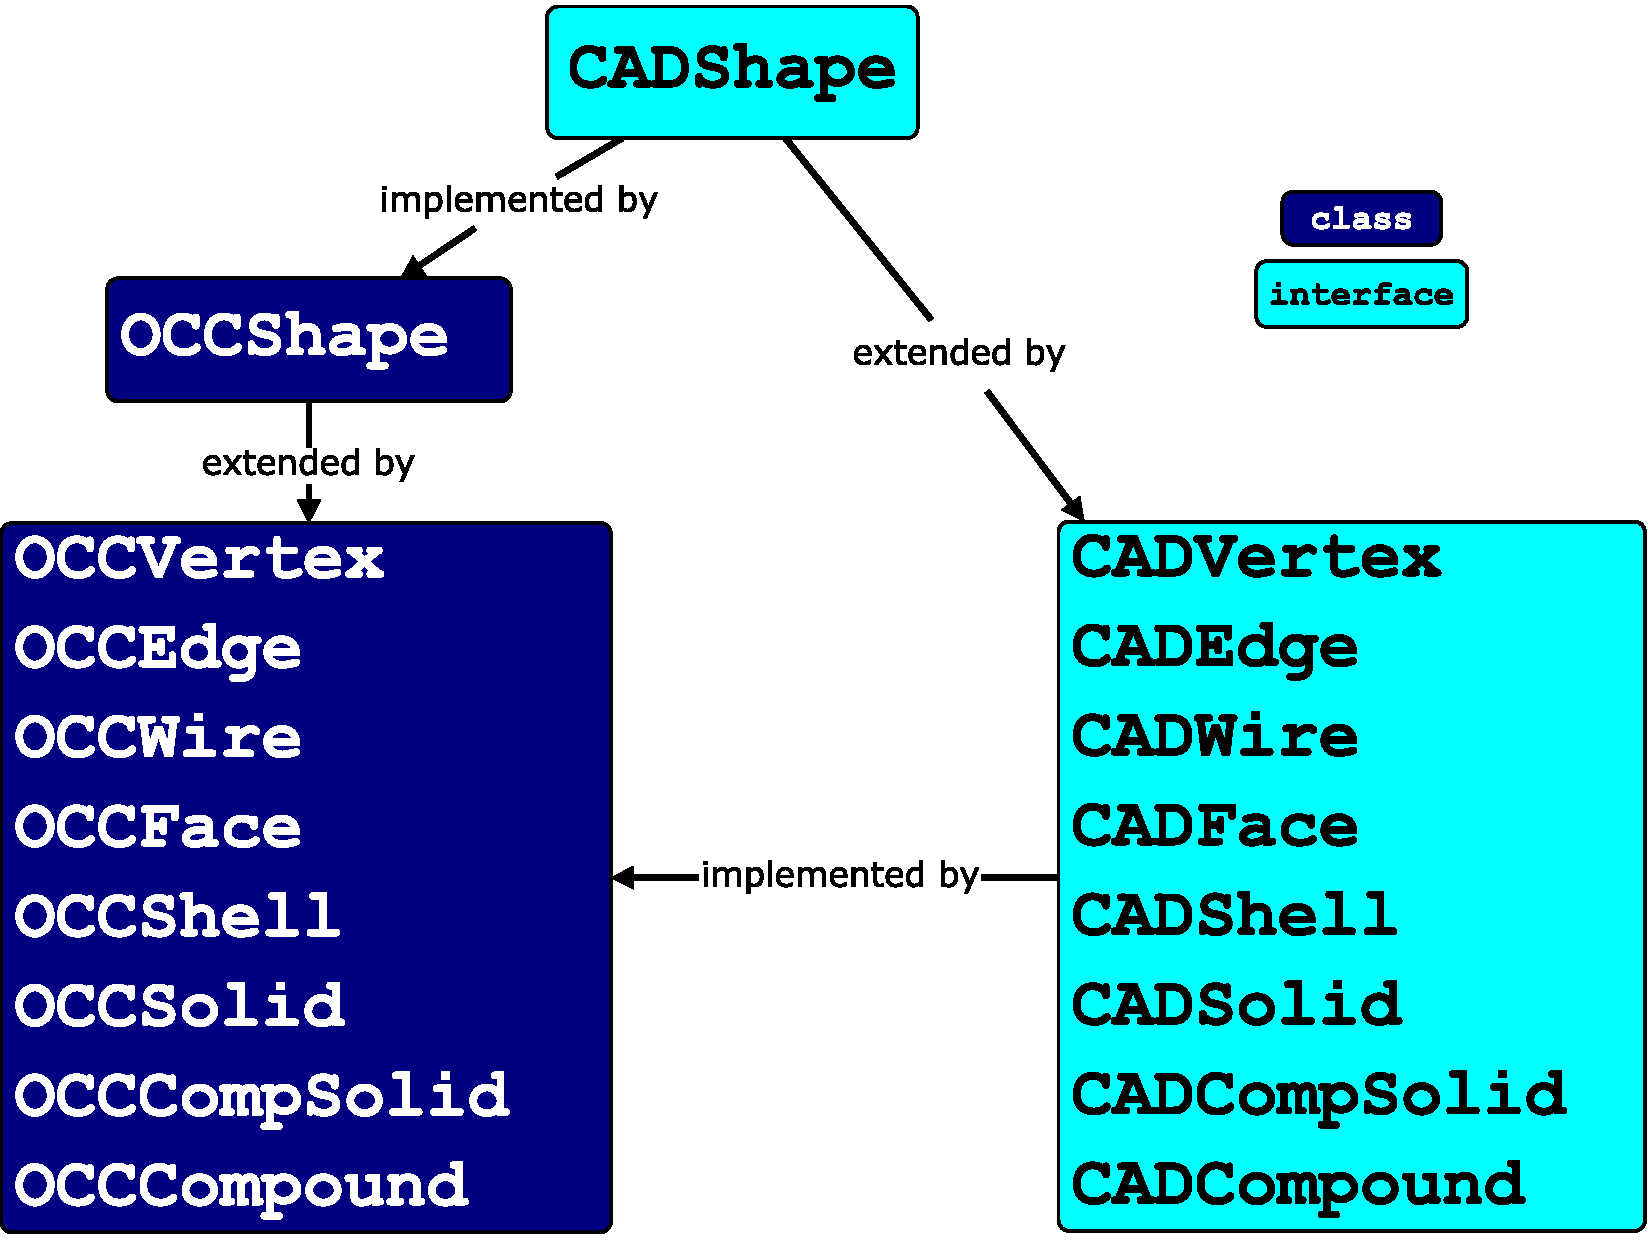
\includegraphics[scale=0.4]{Immagini/Capitolo2/OCCMap}
\caption{Relationship diagram for \lstinline[language=Java]!JPADCAD! topological classes and interfaces}
\label{fig:OCCMap}
\end{figure}
%
\bigskip
\begin{table}[H]
\centering
\begin{tabular}{p{4.2cm}p{10.3cm}}
\toprule
\textbf{Method} & \textbf{Description} \\
\midrule
\lstinline[language=Java]!boundingBox()! & Returns the bounding box of the shape in a \lstinline[language=Java]!double! array format \\[0.2cm]
\lstinline[language=Java]!reversed()! & Returns a reversed instance of the shape \\[0.2cm]
\lstinline[language=Java]!orientation()! & Returns \lstinline[language=Java]!int! value 1 if the shape is forward oriented \\[0.2cm]
\lstinline[language=Java]!isOrientationForward()! & Returns \lstinline[language=Java]!boolean! value \lstinline[language=Java]!true! if the shape is forward oriented \\[0.2cm]
\lstinline[language=Java]!equals(Object o)! & Returns \lstinline[language=Java]!boolean! value \lstinline[language=Java]!true! if \lstinline[language=Java]!o! has same orientation and geometry as the shape \\[0.2cm]
\lstinline[language=Java]!isSame(Object o)! & Returns \lstinline[language=Java]!boolean! value \lstinline[language=Java]!true! if \lstinline[language=Java]!o! has same geometry as the shape \\[0.2cm]
\lstinline[language=Java]!writeNative(String file)! & Writes the shape into the native format \\[0.2cm]
\lstinline[language=Java]!hashCode()! & Returns a hash code matching the equals method \\
\bottomrule
\end{tabular}
\caption{\lstinline[language=Java]!CADShape! methods}
\label{tab:CADShapeMethods}
\end{table}
%
\noindent
As previously stated, \lstinline[language=Java]!OCCShape! generic class implements the \lstinline[language=Java]!CADShape! interface, adding to it also an empty constructor, a shape attribute (of the \lstinline[language=Java]!TopoDS_Shape! type), and setter and getter for the shape attribute. Each \lstinline[language=Java]!OCC! topology class that extends \lstinline[language=Java]!OCCShape! then specifies its own constructors. Listing \ref{lst:shellConstructors} has been included as an example of how shell-type elements can be built, as it reports a partial list of the constructors belonging to this class, plus a private method which provides the actual algorithm through which all the constructors work. The \lstinline[language=Java]!myShape! variable reported in this listing is the previously mentioned shape attribute that each class that extends the \lstinline[language=Java]!OCCShape! one acquires. One thing though should be highlighted: none of the constructors is actually used directly to build new shape objects (as for the shell-type elements as for the others). Following the Abstract Factory pattern, new elements are built through the use of factories and utility classes, as reported in the next paragraphs. 
%
\bigskip
\begin{lstlisting}[caption={\lstinline!OCCShell! constructors and methods}, captionpos=b, tabsize=2, label={lst:shellConstructors}]
public class OCCShell extends OCCShape implements CADShell
{
	// Shell area
	private double area = 0.0;
	
	// Shell builder attributes.
	private static long defaultMakeSolid = 0;
	private static long defaultMakeRuled = 0;
	private static double defaultPrec3D = 1.0e-06;
	
	// Setters and getters
	public static boolean isDefaultMakeSolid() {
			return (defaultMakeSolid == 1);
	}

	public static void setDefaultMakeSolid(boolean value) {
			OCCShell.defaultMakeSolid = (value) ? 1 : 0;
	}

	public static boolean isDefaultMakeRuled() {
			return (defaultMakeRuled == 1);
	}

	public static void setDefaultMakeRuled(boolean value) {
			OCCShell.defaultMakeRuled = (value) ? 1 : 0;
	}

	public static double getDefaultPrec3D() {
			return defaultPrec3D;
	}

	public static void setDefaultPrec3D(double defaultPrec3D) {
			OCCShell.defaultPrec3D = defaultPrec3D;
	}
	
	@Override
	public double getArea() {
			return area;
	}

	// CONSTRUCTORS
	
	/**
	 * Default empty constructor
	 */
	public OCCShell() {
	}	

	/**
	 * Builds a shell through a list of curves
	 */
	public OCCShell(List<CADGeomCurve3D> cadGeomCurveList) {
	
			myShape = OCCShellThruSections(
					null, cadGeomCurveList, null, 
					defaultMakeSolid, defaultMakeRuled, defaultPrec3D
					);
	}

	/**
	 * Builds a shell making it pass through a list of curves and an initial vertex
	 */
	public OCCShell(OCCVertex v0, List<CADGeomCurve3D> cadGeomCurveList) {
	
			myShape = OCCShellThruSections(
					v0, cadGeomCurveList, null, 
					defaultMakeSolid, defaultMakeRuled, defaultPrec3D
					);
	}

	/**
	 * Builds a shell making it pass through a list of curves and a final vertex
	 */
	public OCCShell(List<CADGeomCurve3D> cadGeomCurveList, OCCVertex v1) {
	
			myShape = OCCShellThruSections(
					null, cadGeomCurveList, v1, 
					defaultMakeSolid, defaultMakeRuled, defaultPrec3D
					);
	}
	
	/**
	 * Builds a shell making it pass through a 
	 * list of curves and initial and final vertices
	 */
	public OCCShell(
			OCCVertex v0, List<CADGeomCurve3D> cadGeomCurveList, OCCVertex v1) {
			
			myShape = OCCShellThruSections(
					v0, cadGeomCurveList, v1, 
					defaultMakeSolid, defaultMakeRuled, defaultPrec3D
					);
	}
	
	/**
	 * Actual shell builder, based on OCCT low-level algorithms
	 */
	private TopoDS_Shape OCCShellThruSections(
				OCCVertex v0, List<CADGeomCurve3D> cadGeomCurveList, OCCVertex v1,
				long solid, long ruled, double pres3d) {		
		...
	}
}
\end{lstlisting}
%

\subsubsection{Geometry classes}

\lstinline[language=Java]!JPADCAD! currently comprises six geometry classes, dealing with both 2D and 3D geometric entities. As well as for the shape classes, the \lstinline[language=Java]!CAD! prefix indicates the interfaces dealing with abstract geometry, while the \lstinline[language=Java]!OCC! prefix indicates classes relative to the \gls{OCCT} kernel implementation. Table \ref{tab:JPADCADGeomEnt} gives an overview on the geometry classes contained in \lstinline[language=Java]!JPADCAD!. Another class should be added to this list: \lstinline[language=Java]!OCCDiscretizeCurve3D!. This class, as the name suggests, is pertinent to the \gls{OCCT} implementation and offers support for 3D curves discretization, giving the user the possibility to manipulate curve points.
%
\bigskip
\begin{table}[H]
\centering
\begin{tabular}{ccc}
\toprule
\textbf{Open CASCADE} & \multicolumn{2}{c}{\textbf{JPAD}} \\
& \textbf{Abstract Geometry} & \textbf{Concrete Geometry} \\
\midrule
\lstinline[language=Java]!Geom2dAdaptor_Curve! & \lstinline[language=Java]!CADGeomCurve2D! & \lstinline[language=Java]!OCCGeomCurve2D! \\
\lstinline[language=Java]!GeomAdaptor_Curve! & \lstinline[language=Java]!CADGeomCurve3D! & \lstinline[language=Java]!OCCGeomCurve3D! \\
\lstinline[language=Java]!Geom_Surface! & \lstinline[language=Java]!CADGeomSurface! & \lstinline[language=Java]!OCCGeomSurface! \\
\bottomrule
\end{tabular}
\caption{\lstinline[language=Java]!JPADCAD! geometry classes overview}
\label{tab:JPADCADGeomEnt}
\end{table}
%
\noindent
Basic interfaces contain just the methods, which are then implemented by the \lstinline[language=Java]!OCC! classes by using the \gls{OCCT} functions. These methods are specific for each geometric entity. As an example of this, table \ref{tab:CADGeomSurfMesh} shows the methods contained in \lstinline[language=Java]!CADGeomSurface!, along with a brief description of the operations intended by each one of them.
%
\bigskip
\begingroup
\begin{longtable}[H]{p{5.7cm}p{8.8cm}}
\toprule
\textbf{Method} & \textbf{Description} \\
\midrule
\endfirsthead
%
{\relsize{-1}({\itshape continues from previous page})} & \\
\toprule
\textbf{Method} & \textbf{Description}\\
\midrule
\endhead
%
\midrule 
{\relsize{-1}({\itshape continues on next page})} & 
\endfoot
%
\bottomrule
\caption{\lstinline[language=Java]!CADGeomSurface! methods}
\endlastfoot
%
\lstinline[language=Java]!dinit(int degree)! & Initializes the degree of the surface \\[0.5cm]
\lstinline[language=Java]!value(double u, double v)! & Gets 3D coordinates from $(\text{u}, \text{v})$ coordinates \\[0.5cm]
\lstinline[language=Java]!lowerDistance(double[] p)! & Returns the distance of a point from the surface \\[0.5cm]
\lstinline[language=Java]!setParameter(double u, double v)! & Sets the $(\text{u}, \text{v})$ coordinates used for derivative and curvature operations \\[0.2cm]
\lstinline[language=Java]!d1U()! & Returns the u first derivative vector at the coordinates set by \lstinline[language=Java]!setParameter! \\[0.2cm]
\lstinline[language=Java]!d1V()! & Returns the v first derivative vector at the coordinates set by \lstinline[language=Java]!setParameter! \\[0.2cm]
\lstinline[language=Java]!d2U()! & Returns the u second derivative vector at the coordinates set by \lstinline[language=Java]!setParameter! \\[0.2cm]
\lstinline[language=Java]!d2V()! & Returns the v second derivative vector at the coordinates set by \lstinline[language=Java]!setParameter! \\[0.2cm]
\lstinline[language=Java]!dUV()! & Returns the cross derivative vector at the coordinates set by \lstinline[language=Java]!setParameter! \\[0.2cm]
\lstinline[language=Java]!normal()! & Returns the normal to the surface at the coordinates set by \lstinline[language=Java]!setParameter! \\[0.2cm]
\lstinline[language=Java]!minCurvature()! & Returns the minimum curvature at the coordinates set by \lstinline[language=Java]!setParameter! \\[0.2cm]
\lstinline[language=Java]!maxCurvature()! & Returns the maximum curvature at the coordinates set by \lstinline[language=Java]!setParameter! \\[0.2cm]
\lstinline[language=Java]!gaussianCurvature()! & Returns the Gaussian curvature at the coordinates set by \lstinline[language=Java]!setParameter! \\[0.2cm]
\lstinline[language=Java]!meanCurvature()! & Returns the mean curvature at the coordinates set by \lstinline[language=Java]!setParameter! \\[0.2cm]
\lstinline[language=Java]!curvatureDirections()! & Returns the direction of maximum and minimum curvature at the coordinates set by \lstinline[language=Java]!setParameter!
\label{tab:CADGeomSurfMesh}
\end{longtable}
\endgroup
%
\bigskip
\noindent
Constructors are implemented by the \lstinline[language=Java]!OCC! classes. The most important of these constructors reside in \lstinline[language=Java]!OCCGeomCurve3D!, since the construction of main aircraft components 3D models starts from a series of curves, quite always provided by a good selection of points read from file. \lstinline[language=Java]!OCCGeomCurve3D! actually features three types of constructor, which are partially reported in listing \ref{lst:OCCGC3DCnst} along with some of the attributes and methods of the class. These constructors use classes belonging to the \gls{OCCT} library. In particular, the constructors based on provided point lists perform interpolation through a crucial \gls{OCCT} class, which is \lstinline[language=Java]!GeomAPI_Interpolate!. This class is used to interpolate a B-Spline curve passing through an array of points, with a C2 continuity if tangency is not requested at any middle point. If tangency is requested at some point the continuity will be C1. If periodicity is requested the curve will be closed and the junction will be the first point given.
%
\bigskip
\begin{lstlisting}[caption={\lstinline!OCCGeomCurve3D! constructors}, captionpos=b, tabsize=2, label={lst:OCCGC3DCnst}]
public class OCCGeomCurve3D implements CADGeomCurve3D
{
	// Attributes
	private CADEdge cadEdge = null;
	private GeomAdaptor_Curve myCurve = null;
	private final double[] range = new double[2];
	private OCCDiscretizeCurve3D discret = null;
	private double length = 0.0;
	
	/**
	 * Returns a point on the curve
	 */
	public double[] value(double p) {
			...
	}
	
	/**
	 * Discretizes myCurve splitting it in n arcs. The result is put into discret
	 */
	public void discretize(int n) {		
			...
	}
	
	/**
	 * Returns myCurve range
	 */
	public double[] getRange() {
			return range
	}
	
	/**
	 * Returns myCurve length
	 */
	public double length() {	
			return length;
	}

	/**
	 * Returns the edge element represented by myCurve
	 */
	public CADEdge edge() {	
			return cadEdge;
	}
	
	/**
	 * Returns myCurve
	 */
	public GeomAdaptor_Curve getAdaptorCurve() {	
			return myCurve;
	}
	
	/**
	 * Returns the discretized curve obtained from discretize method
	 */
	public OCCDiscretizeCurve3D getDiscretizedCurve() {	
			return discret;
	}

	// CONSTRUCTORS
	
	/**
	 * Builds a 3D curve from an edge object
	 */
	public OCCGeomCurve3D(CADEdge E) {	
			...
	}
	
	/**
	 * Builds a 3D curve from a list of double[] points. The second  
	 * parameter tells the method whether the curve is periodic or not.
	 */
	public OCCGeomCurve3D(List<double[]> pointsList, boolean isPeriodic) {	
			...	
	}
	
	/**
	 * Builds a 3D curve from a list of double[] points. The second parameter tells 
	 * the method whether the curve is periodic or not, while the third and fourth
	 * parameter set the initial and final tangents, respectively. The last parameter 
	 * tells the method whether the tangents need to be scaled or not. 
	 */
	public OCCGeomCurve3D(List<double[]> pointList, 
			boolean isPeriodic, 
			double[] initialTangent, double[] finalTangent, 
			boolean doScale) {			
			...
	}
}
\end{lstlisting}
%

\subsubsection{Factory and Utility classes}

Factories and utilities are the classes that are actually exploited by \lstinline[language=Java]!JPADCAD! users in order to instantiate new geometric or topological entities. These classes use the aforementioned constructors to build new \gls{CAD} objects. The abstract factory \lstinline[language=Java]!CADShapeFactory! provides the methods that the concrete factory classes must implement. Currently, \lstinline[language=Java]!OCCShapeFactory! is the only implementation provided in \lstinline[language=Java]!JPADCAD!, allowing the construction of 3D \gls{CAD} entities by the use of the \gls{OCCT} classes. Below there is a list of the methods provided by the \lstinline[language=Java]!CADShapeFactory!, along with a description of what they do and the constructors they make use of in the \gls{OCCT} implementation.
%
\begin{itemize}
\renewcommand\labelitemi{\tiny$\blacksquare$}
\renewcommand\labelitemii{\tiny$\bullet$}
\item \textbf{\lstinline[language=Java]!getFactory!, \lstinline[language=Java]!setFactory!} - Getter and setter for the \lstinline[language=Java]!CADShapeFactory! attribute \lstinline[language=Java]!factory!. This attribute needs to be instantiated one time, whenever factory methods are needed.
\item \textbf{\lstinline[language=Java]!newExplorer!, \lstinline[language=Java]!newWireExplorer!} - Methods through which new instances for generic topology explorer (\lstinline[language=Java]!CADExplorer!) and wire explorer (\lstinline[language=Java]!CADWireExplorer!) are created. These explorers are intended for topological data structure investigation. In case of a generic explorer, the shape to explore and the type of the shapes to be found must be provided.
\item \textbf{\lstinline[language=Java]!newIterator!} - Creates a \lstinline[language=Java]!CADIterator! object, intended for sub-shapes iteration.
\item \textbf{\lstinline[language=Java]!newShape!} - Methods that generate \lstinline[language=Java]!CADShape! generic entities. The input provided to the method can be:
	\begin{itemize}
	\item a generic \lstinline[language=Java]!Object! of the underlying implementation (e.g., a \lstinline[language=Java]!TopoDS_Edge! object);
	\item a \lstinline[language=Java]!String! standing for the path to a file, from which \gls{CAD} shapes need to be loaded;
	\item a pair of \lstinline[language=Java]!CADShape! objects and a \lstinline[language=Java]!char!, in order to perform Boolean operations.
	\end{itemize}
In the \gls{OCCT} implementation, Boolean operations are performed thanks to the classes contained in the \lstinline[language=Java]!BRepAlgoAPI! package. The \lstinline[language=Java]!char! parameter allows the user to select the type of the operation to be performed.
\item \textbf{\lstinline[language=Java]!newCurve2D!} - Creates a \lstinline[language=Java]!CADGeomCurve2D! object. Currently the factory contains just one method for 2D curves construction, which needs as input the edge owning the 2D curve and the face (i.e., the plane) containing the same curve.
\item \textbf{\lstinline[language=Java]!newCurve3D!} - Methods used to create \lstinline[language=Java]!CADGeomCurve3D! objects, exploiting the constructors reported in listing \ref{lst:OCCGC3DCnst}. These constructors (and so these methods) allow to generate 3D curves starting from:
	\begin{itemize}
	\item an edge owning the 3D curve;
	\item a pair of points in \lstinline[language=Java]!double[]! format (in order to generate a segment);
	\item an indefinite number (at least two elements) of points in \lstinline[language=Java]!double[]! format;
	\item a list of points in \lstinline[language=Java]!double[]! format;
	\item a list of points in \lstinline[language=Java]!double[]! format, and initial and final tangents in terms of \lstinline[language=Java]!double[]!;
	\item a list of \lstinline[language=Java]!gp_Pnt! (an \gls{OCCT} class used to represent points in 3D space);
	\item a list of \lstinline[language=Java]!PVector! (a class, part of the Java Processing package, which describes two or three dimensional vectors \cite{PVector}).
	\end{itemize}
All the aforementioned methods that generate a 3D curve from points assignment also allow the user to set the curve as periodic.
\item \textbf{\lstinline[language=Java]!newVertex!} - Generates new vertices by providing coordinates in terms of \lstinline[language=Java]!double!.
\item \textbf{\lstinline[language=Java]!newFacePlanar!} - Methods that allow to generate a \lstinline[language=Java]!CADFace! as a planar triangle connecting three vertices. The vertices can be provided both in terms of \lstinline[language=Java]!double[]! points and \lstinline[language=Java]!OCCVertex! entities.
\item \textbf{\lstinline[language=Java]!newShell!} - These methods help the user to build a shell, making it pass through a selected list of curves, and initial and final vertices eventually. The \lstinline[language=Java]!OCCShell! constructors actually allowing the necessary operations have been reported in listing \ref{lst:shellConstructors}. In particular, the \lstinline[language=Java]!newShell! methods enable the user to generate shell elements from the following inputs:
	\begin{itemize}
	\item a list of \lstinline[language=Java]!CADGeomCurve3D!;
	\item an initial \lstinline[language=Java]!CADVertex!, a list of \lstinline[language=Java]!CADGeomCurve3D!, one final \lstinline[language=Java]!CADVertex!.
	\end{itemize}
The \gls{OCCT} class \lstinline[language=Java]!BRepOffsetAPI_ThruSections! provides the algorithms to perform \lstinline[language=Java]!newShell! underlying operations. This class describes functions to build a loft (a shell or a solid entity) passing through a set of sections in a given sequence. It is necessary to point out that none of these methods is used directly to generate shell elements: the \lstinline[language=Java]!OCCUtils! utility class actually contains the methods used in practice, as it will be clear shortly. 
\item \textbf{\lstinline[language=Java]!newShellFromAdjacentFaces!} - It allows to build a shell by connecting adjacent faces. Faces can be provided both in an array of indefinite lenght and in a list. The algorithms that perform the operations in the \gls{OCCT} implementation are provided by the \lstinline[language=Java]!BRepBuilderAPI_Sewing! class.
\item \textbf{\lstinline[language=Java]!newSolidFromAdjacentFaces!} - Performs the same operations described above, producing a solid instead of a shell. In the \gls{OCCT} implementation, the solid is produced by the use of the \lstinline[language=Java]!BRepBuilderAPI_MakeSolid! class.
\end{itemize}
%

\bigskip
\noindent
The concrete factory class \lstinline[language=Java]!OCCShapeFactory!, as long as its methods, are not intended to be instantiated and exploited directly by \lstinline[language=Java]!JPADCAD! users. The utility class \lstinline[language=Java]!OCCUtils!, instead, is intended to be used in order to generate new factory instances through which factory methods can be performed. In particular, \lstinline[language=Java]!OCCUtils! gives the user the capability to make the following operations.
%
\begin{enumerate}
\item Generate a new \lstinline[language=Java]!OCCShapeFactory! instance and assigning it to its own \lstinline[language=Java]!theFactory! attribute, which belongs to the \lstinline[language=Java]!CADShapeFactory! type.
\item Access factory methods through \lstinline[language=Java]!theFactory! attribute, performing the operations on shapes listed above.
\end{enumerate}
%
In addition, \lstinline[language=Java]!OCCUtils! contains several methods covering different necessities that can be encountered while managing \gls{CAD} entities. Though some of these functions just make use of factory methods by simply rearranging the way their parameters are set (as for the methods making use of \lstinline[language=Java]!newShell! factory functions), others allow the users to perform completely new manipulation operations on shapes. Obviously, the methods contained in this utility, as well as the utility class itself, are inherent to the \gls{OCCT} implementation. The following list offers an overview on the methods contained in \lstinline[language=Java]!OCCUtils!.
%
\begin{itemize}
\renewcommand\labelitemi{\tiny$\blacksquare$}
\item \textbf{\lstinline[language=Java]!write!} methods allow to write produced shapes to file. In order to be exported, shapes must be \lstinline[language=Java]!OCCShape! generic instances. The methods currently contained in \lstinline[language=Java]!OCCUtils! allow to write shapes just in BRep format. Other formats, such as STEP and IGES, are actually covered in another utility class, \lstinline[language=Java]!AircraftUtils!, which, at the moment, is contained in \lstinline[language=Java]!JPADCADSandbox!, and whose methods will be explained in the next chapters.
\item \textbf{\lstinline[language=Java]!reportOnShape!} and \textbf{\lstinline[language=Java]!numberOfShapes!} methods enable to investigate shapes, providing a report (viewable on console) on the sub-shapes and their number.
\item \textbf{\lstinline[language=Java]!pointProjectionOnCurve!} methods enable to project points onto a 3D curve, providing \lstinline[language=Java]!CADVertex! entities as result. The \gls{OCCT} class \lstinline[language=Java]!GeomAPI_ProjectPointOnCurve! is behind this operation.
\item \textbf{\lstinline[language=Java]!splitEdge!} functions allow to split edges or curves at one or more locations, returning a list of \lstinline[language=Java]!CADEdge! entities as result. The Open CASCADE class underlying the operations performed by these methods is \lstinline[language=Java]!BOPAlgo_PaveFiller!.
\item \textbf{\lstinline[language=Java]!makeFilledFace!} methods allow the user to generate filling surfaces, i.e., surfaces that can be used to fill empty gaps between faces. These methods make use of the \gls{OCCT} class \lstinline[language=Java]!BRepOffsetAPI_MakeFilling! and \lstinline[language=Java]!newShape! factory methods.
\item \textbf{\lstinline[language=Java]!makePatchThruSections!} routines, finally, make use of \lstinline[language=Java]!newShell! factory methods, in order to enhance user possibilities in terms of which type of parameters can be provided as input in order to generate a shell element from a sequence of points and curves.
\end{itemize}
%

\bigskip
\noindent
The following paragraph shows some simple examples on how \lstinline[language=Java]!JPADCAD! classes are used in order to produce basic shapes. The next chapter will deal on how all the aforementioned methods can be used in order to generate shapes representing more complex geometries, such as those behind main aircraft components.

\subsection{Examples}
\label{sec2.3.3}

The following example shows how to generate B-Spline curves and loft surfaces in \lstinline[language=Java]!JPADCAD!. The methods used below are those descripted in the previous paragraph. Some particular attention has been put on such methods because they are among the most used for aircraft components \gls{CAD} models production. 

\bigskip
\noindent
As previously explained, in order to be able to actually generate \gls{CAD} shapes in \gls{JPAD} it is necessary to instantiate a factory. For this reason, the first method called through \lstinline[language=Java]!OCCUtils! is \lstinline[language=Java]!initCADShapeFactory!. After making sure that a \lstinline[language=Java]!OCCShapeFactory! instance actually exists, the first thing to do is creating points for the curves. In the listing below, these points are created in \lstinline[language=Java]!double[]! format, and passed to the \lstinline[language=Java]!newCurve3D! method, along with a \lstinline[language=Java]!boolean! value that states that the curve we want to generate is not periodic. The application of the previous method returns a generic \lstinline[language=Java]!CADGeomCurve3D!, as required by the use of the Abstract Factory pattern. Exploiting the \lstinline[language=Java]!edge! method provided by the \lstinline[language=Java]!CADGeomCurve3D! interface, the \lstinline[language=Java]!CADEdge! entity underlying the B-Spline curve can be obtained.
%
\bigskip
\begin{lstlisting}[caption={B-Spline curve creation}, captionpos=b, tabsize=2, label={lst:Example1}]		
		if(OCCUtils.theFactory == null) 
			OCCUtils.initCADShapeFactory();
		
		// Create a list of points to be passed to the 
		// factory methods for 3D curves generation
		double[] pntA = new double[] {0.0, -1.0, 0.0};
		double[] pntB = new double[] {0.0,  0.0, 1.0};
		double[] pntC = new double[] {0.0,  2.0, 0.0};
		
		// Generate a B-Spline curve from the previous points
		CADGeomCurve3D curve1 = OCCUtils.theFactory.newCurve3D(false, pntA, pntB, pntC);
		
		// Get the edge entity underlying the previous curve
		CADEdge edge1 = curve1.edge();
\end{lstlisting}
%
\bigskip
\noindent
In order to produce other curves and to show how \lstinline[language=Java]!newCurve3D! can actually manage more than just one set of parameters (thanks to Java polymorphism), the previous points are added to a Java \gls{List} \cite{JavaList} and manipulated (after being inserted in the list), in order to generate the successive curves at a certain distance from the previous one. In this way, two more curves are made, with the last one being also imposed two tangency constraints, at the initial and final point respectively. Once all the curves are made, the \lstinline[language=Java]!write! method is called by the use of \lstinline[language=Java]!OCCUtils!, allowing to write the desired shapes to a BRep file. The result is shown in figure \ref{fig:EdgeExample}.
%
\bigskip
\begin{lstlisting}[caption={B-Spline curve creation with different \lstinline!newCurve3D! methods}, captionpos=b, tabsize=2, label={lst:Example2}]		
		// Passing points to the B-Spline curves generator method through a Java List
		List<double[]> points1 = new ArrayList<double[]>();
		
		points1.add(pntA);
		points1.add(pntB);
		points1.add(pntC);		
		points1.forEach(d -> d[0] = 2.0);
		
		CADGeomCurve3D curve2 = OCCUtils.theFactory.newCurve3D(points1, false);
		
		// Get the edge entity underlying the previous curve
		CADEdge edge2 = curve2.edge();
		
		// Give to the B-Spline factory method initial and final tangent too
		List<double[]> points2 = new ArrayList<double[]>();
		
		points2.addAll(points1);
		points2.forEach(d -> d[0] = 10.0);
		
		double[] iTang = new double[] {0.0, 1.0, 0.0};
		double[] fTang = iTang;
		
		CADGeomCurve3D curve3 = OCCUtils.theFactory.newCurve3D(points2, 
				false, 
				iTang, fTang, 
				false
				);
		
		// Get the edge entity underlying the previous curve
		CADEdge edge3 = curve3.edge();
		
		// Writing the generated edges to BRep file
		System.out.println("Have been the shapes correctly written to file? " + 
				OCCUtils.write("EdgeExample_01.brep", 
						(OCCEdge) edge1, 
						(OCCEdge) edge2,
						(OCCEdge) edge3
						));
\end{lstlisting}
%
\bigskip
\noindent
The last part of the example focuses on \lstinline[language=Java]!newShell! and \lstinline[language=Java]!makePatchThruSections! methods. The curves used as sections for the loft are those created in the first part of the example. Three lofts are made, exploiting three \lstinline[language=Java]!makePatchThruSections! available variants. The example also shows how to generate \lstinline[language=Java]!CADVertex! entities by use of a \lstinline[language=Java]!double! array. Generated shapes are then transcripted to file and reported in figures \ref{fig:ShellExample1}, \ref{fig:ShellExample2} and \ref{fig:ShellExample3}.
%
\bigskip
\begin{lstlisting}[caption={Lofts creation by use of \lstinline!makePatchThruSections! methods}, captionpos=b, tabsize=2, label={lst:Example3}]	
		// Making a shell pass through the curves
		OCCShape shell1 = OCCUtils.makePatchThruSections(curve1, curve2, curve3);
		
		// Writing the generated shell to BRep file
		System.out.println("Have been the shapes correctly written to file? " + 
				OCCUtils.write("ShellExample_01.brep", shell1));
					
		// Making a shell pass through the above generated curves and an initial vertex
		List<CADGeomCurve3D> curves = new ArrayList<CADGeomCurve3D>();
		
		curves.add(curve1);
		curves.add(curve2);
		curves.add(curve3);
		
		CADVertex iVtx = OCCUtils.theFactory.newVertex(new double[] {-10.0, 0.0, 0.0});
		
		OCCShape shell2 = OCCUtils.makePatchThruSections(iVtx, curves);
		
		// Writing the generated shell to BRep file
		System.out.println("Have been the shapes correctly written to file? " + 
				OCCUtils.write("ShellExample_02.brep", shell2));
		
		// Making a shell pass through initial and final vertices too
		CADVertex fVtx = OCCUtils.theFactory.newVertex(new double[] {20, 0.0, 0.0});

		OCCShape shell3 = OCCUtils.makePatchThruSections(iVtx, curves, fVtx);

		// Writing the generated shell to BRep file
		System.out.println("Have been the shapes correctly written to file? " + 
				OCCUtils.write("ShellExample_03.brep", shell3));		
\end{lstlisting}
%
\begin{figure}[!ht]
\centering
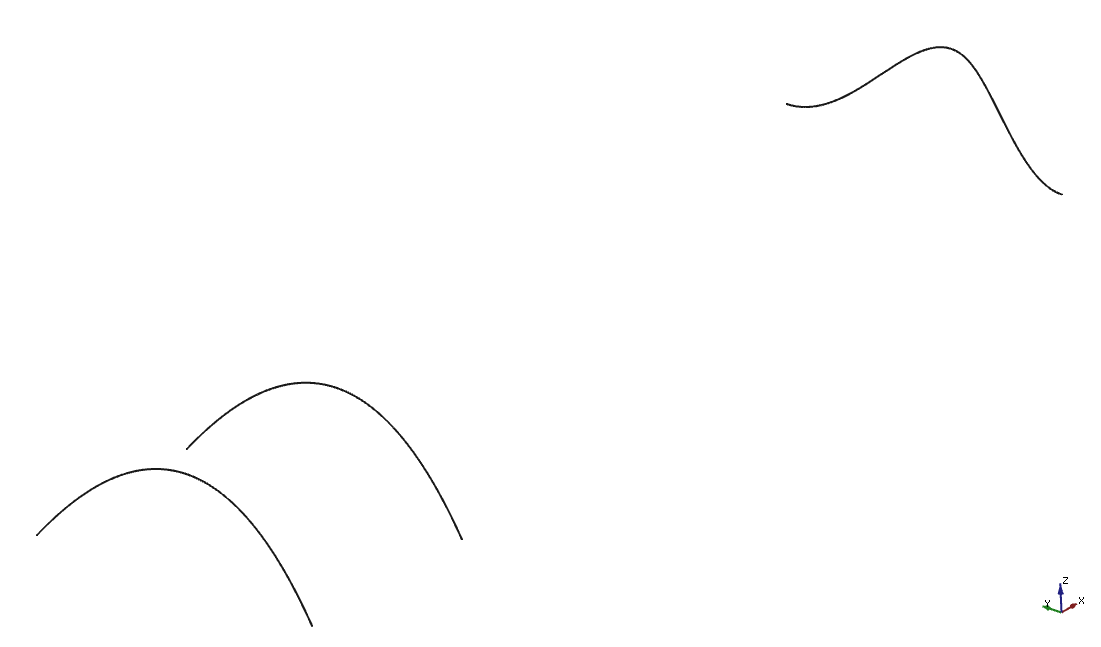
\includegraphics[scale=0.5]{Immagini/Capitolo2/EdgeExample2}
\caption{Edges obtained by use of \lstinline[language=Java]!newCurve3D! methods}
\label{fig:EdgeExample}
\end{figure}
%
%
\begin{figure}[!ht]
\centering
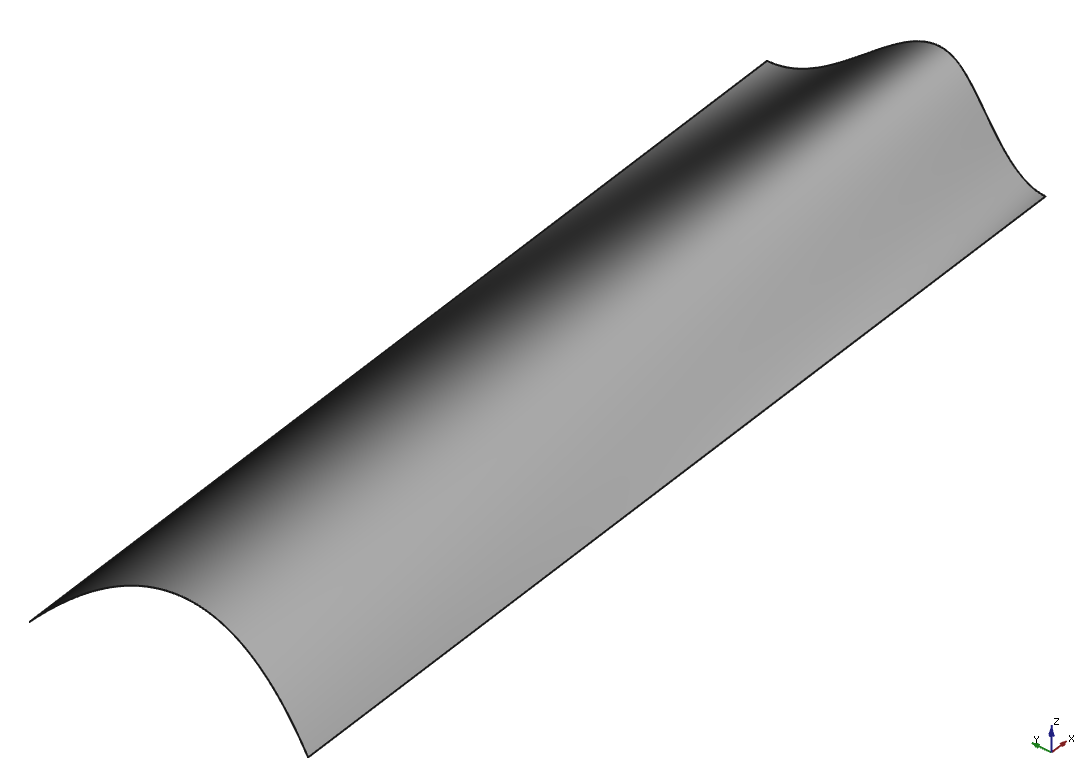
\includegraphics[scale=0.5]{Immagini/Capitolo2/ShellExample12}
\caption{Loft passing through three curves}
\label{fig:ShellExample1}
\end{figure}
%
%
\begin{figure}[!ht]
\centering
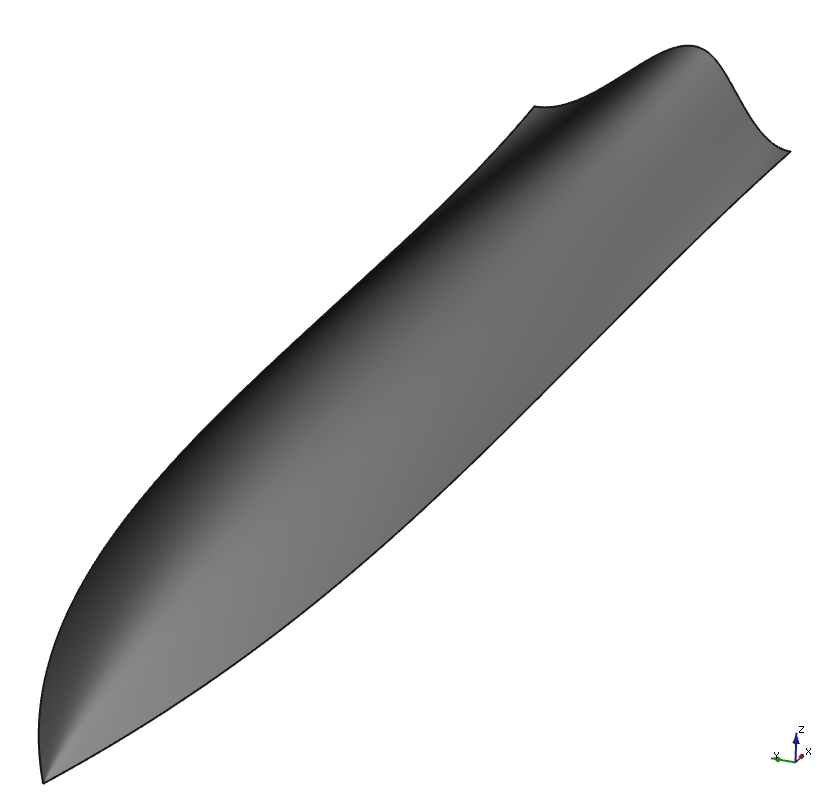
\includegraphics[scale=0.6]{Immagini/Capitolo2/ShellExample22}
\caption{Loft passing through three curves and an initial vertex}
\label{fig:ShellExample2}
\end{figure}
%
%
\begin{figure}[!ht]
\centering
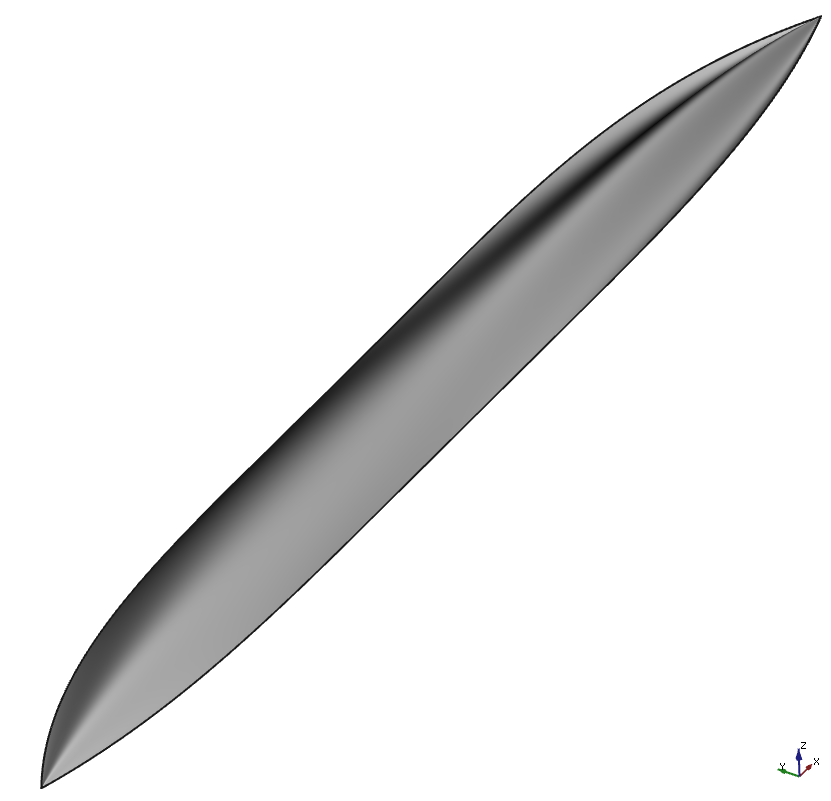
\includegraphics[scale=0.6]{Immagini/Capitolo2/ShellExample32}
\caption{Loft passing through three curves and initial and final vertices}
\label{fig:ShellExample3}
\end{figure}
%